\subsection{Zadania}

\setcounter{problem}{0}

\begin{problem}
  Niech $\{X_n\}$ będzie martyngałem. Uzasadnij wykładniczą wersję nierówności Dooba: dla każdego $h>0$ i każdego $n\in\N$
  $$\prob{\max X_k>x}\leq e^{-hx}\expected{e^{hX_n}}$$
\end{problem}

\begin{solution}
  Rozważmy czas zatrzymania
  $$T=\inf\{k\;:\;X_k>x\}$$
  dowód wygląda podobnie jak dowód twierdzenia \ref{max slabego}:
  \begin{align*}
    \expected{e^{hX_n}}&\geq \expected{e^{hX_{n\land T}}}=\expected{e^{hX_{n\land T}}\mathds{1}_{\{\max X_k >x\}}} + \expected{e^{hX_{n\land T}}\mathds{1}_{\{\max X_k\leq x\}}}= \\ 
    &= \expected{e^{hX_T}\mathds{1}_{\{\max X_k>x\}}}+\expected{e^{hX_n}\mathds{1}_{\{\max X_k\leq x\}}}\geq \expected{e^{hx}\mathds{1}_{\{\max X_k>x\}}}=\\ 
    &=e^{hx}\expected{\mathds{1}_{\{\max X_k>x\}}}=e^{hx}\prob{\max X_k>x}
  \end{align*}
  czyli po przerzuceniu $e^{hx}$ na lewą stronę, dostajemy tezę.
\end{solution}

\begin{problem}
  Niech $\{X_n\}$ będzie martyngałem całkowalnym z kwadratem ($\expected{X_n^2}<\infty$ dla każdego $n\in\N$). Pokaż, że
  $$\expected{(X_n-X_m)^2}{\set{F}_m}=\expected{X_n^2}{\set{F}_m}-X_m^2$$
  {\color{red}Dodatkowe założenia: $n>m$.}
\end{problem}

\begin{solution}
  Po pierwsze, wypadałoby pokazać, że $X_nX_m$ jest całkowalne
  $$\expected{|X_nX_m|}\leq\expected{|X_n|^2}^{1/2}\expected{|X_m|^2}^{1/2}<\infty$$
  W takim razie, wiedząc, że $X_m$ jest zawsze mierzalna względem $\set{F}_m$ wiemy, że $\expected{X_nX_m}{\set{F}_m}=X_m\expected{X_n}{\set{F}_m}$ i teraz jeśli $n>m$ to i $\expected{X_n}{\set{F}_m}=X_m$, co pokazaliśmy już dawno temu na liście. Przechodząc z tą wiedzą do pisania, mamy;
  \begin{align*}
    \expected{(X_n-X_m)^2}{\set{F}_m}&=\expected{X_n^2-2X_nX_m+X_m^2}{\set{F}_m}=\\ 
                                     &=\expected{X_n^2}{\set{F}_m}+\expected{X_m^2}{\set{F}_m}-2X_m\expected{X_n}{\set{F}_m}=\\ 
                                     &=\expected{X_n^2}{\set{F}_m}+X_m^2-2X_m^2=\expected{X_n^2}{\set{F}_m}-X_m^2
  \end{align*}
\end{solution}

\begin{problem}
  Niech $\{Z_n\}$ będzie procesem Galtona-Watsona dla którego $\expected{Z_1}=\mu$ oraz $Var(Z_1)=\sigma^2<\infty$. Rozważmy martyngał $M_n=\mu^{-n}Z_n$.
  \begin{enumerate}[label=(\alph*)]
    \item Pokaż, że
      $$\expected{M_n^2}=1+\sigma^2\sum_{k=2}^{n+1}\mu^{-k}$$
    \item Uzasadnij, że jeśli $\mu>1$, to $M_n$ jest zbieżny w $L^2$
    \item Uzasadnij, że jeśli $\mu<1$, to $M_n$ nie jest zbieżny w $L^2$.
  \end{enumerate}
\end{problem}

\begin{solution}
  Proces Galtona-Watsona pojawił się w rozdziale \ref{procel galtona-watsona}, gdy chcieliśmy obserwować pantofelki rozmnażające się bezpłciowo, niezależnie od siebie. Rozważaliśmy zmienne losowe $Y_{n,k}$ takie oraz ciąg
  $$Z_1=1$$
  $$Z_{n+1}=\sum_{k=1}^{Z_n}Y_{n+1,k}$$
  gdzie $Z_n$ to liczba nowych pantofelków w $n$-tej generacji, a $Y_{n,k}$ to liczba potomstwa w $n$-tej generacji zrodzona przez $k$-tego pantofelka w $n-1$ generacji.

  \begin{enumerate}[label=(\alph*)]
    \item Wiem już, że
      $$\expected{Z_1}=\expected{\sum_{k=1}^{Z_0}Y_{n,k}}=\expected{Y_{1,1}}=\mu$$
      oraz (korzystając z tego co pokazaliśmy na wykładzie):
      $$\expected{Z_{n+1}}=\expected{Y_{n,k}}\expected{Z_n}=\mu\expected{Z_n}=\mu^{n+1}.$$

      Całość pokażemy za pomocą indukcji. Jeśli $n=1$, to mamy
      $$\expected{M_1^2}=\expected{\mu^{-2}Z_1^2}=\mu^{-2}\expected{Z_1^2}=\mu^{-2}[Var(Z_1)+\expected{Z_1}^2]=\sigma^2\mu^{-2}+1$$
      tak jak chcieliśmy.

      Zróbmy teraz krok indukcyjny, czyli $n\implies n+1$. Będziemy korzystać z zadania 2, więc chcemy wyliczyć $M_{n+1}-M_n$
      \begin{align*}
        M_{n+1}-M_n&=\mu^{-n-1}\sum_{k=1}^{Z_{n}}Y_{n,k}-\mu^{-n}Z_n=\mu^{-n-1}\sum_{k=1}^{Z_n}(Y_{n,k}-\mu)
      \end{align*}
      Wstawiając do równości w zadaniu 2 (po scałkowaniu), dostajemy
      \begin{align*}
        \expected{M_{n+1}^2}&=\expected{(M_{n+1}-M_n)^2}+\expected{M_{n}^2}=\\ 
                            &=\expected{\left( \mu^{-n-1}\sum_{k=1}^{Z_n}(Y_{n,k}-\mu) \right)^2} +1+\sigma^2\sum_{k=2}^{n+1}\mu^{-k}=\\ 
                            &=\mu^{-2n-2}\expected{\left(\sum_{k=1}^{Z_n}(Y_{n,k}-\mu)\right)^2}+1+\sigma^2\sum_{k=2}^{n+1}\mu^{-k}=(\star)
      \end{align*}
      Pozostaje pokazać, że $\expected{\left(\sum_{k=1}^{Z_n}(Y_{n,k}-\mu)\right)^2}=\mu^{n}\sigma^2$.

      Rozważmy funkcję 
      \begin{align*}
        h(z)&=Var(\sum_{k=1}^zY_{n+1,k})=\expected{\left(\sum_{k=1}^zY_{n+1,k}-z\mu\right)^2}=\\ 
            &=\sum_{k=1}^zVar(Y_{n+1,k})=zVar(Y_{1,1})=zVar(Z_1)=z\sigma^2
      \end{align*}
      i zauważmy, że wwo
      $$\expected{\left(\sum_{k=1}^{Z_n}(Y_{n+1,k}-\mu)\right)^2}{\set{F}_n}=h(Z_n)=Z_n\sigma^2$$
      czyli całkując obie strony otrzymujemy
      $$\expected{\left(\sum_{k=1}^{Z_n}(Y_{n+1,k}-\mu)\right)^2}=\expected{Z_n\sigma^2}=\mu^n\sigma^2$$
      i to jest tym co chcieliśmy, bo wracając do kroku indukcyjnego
      $$(\star)=\mu^{-n-2}\mu^n \sigma^2+1+\sigma^2\sum_{k=2}^{n+1}\mu^{-k}=1+\sigma^2\sum_{k=2}^{n+2}\mu^{-k}$$
    \item Aby $M_n$ zbiegało w $L^2$, musimy znaleźć funkcję $X$ taką, że $\expected{|M_n-X|^2}\to 0$. Zauważmy, że $Z_n$ zawsze przyjmuje skończone wartości, czyli $M_n=\mu^{-n}Z_n\to 0$, bo $\mu^{-n}\to 0$. W takim razie mamy $X=0$ jest potencjalną granicą $M_n$. Wystarczy wyliczyć
      \begin{align*}
        \expected{|M_n|^2}&=1+\sigma^2\sum_{k=2}^{n+1}\mu^{-k}=1+\sigma^2\sum_{k=0}^{n-1}\mu^{-k-2}=\\ 
                          &=1+\sigma^2\mu^{-2}\sum_{k=0}^{n-1}\mu{-k}=1+\sigma^2\mu^{-2}\sum_{k=0}^{n-1}\mu^{-k}=\\ 
                          &=1+\sigma^2\mu^{-2}\frac{1-\mu^{-n}}{1-\mu^{-1}}=1+\sigma^2\mu^{-1}\frac{1-\mu^{-n}}{\mu-1}\leq 1+\sigma^2\mu^{-1}\frac{1}{\mu-1}<\infty
      \end{align*}
      czyli stosuje się do tego twierdzenie \ref{tw 7.5}, ponieważ spełniony jest warunek $\sup\expected{|M_n|^p}<\infty\iff$ istnieje $M_\infty$ że $M_n\to M_\infty$ w $L^p$ dla $p=2$.
    \item Argument jest prawie taki sam jak wyżej, z tym, że
      $$\expected{|M_n|^2}=1+\sigma^2\mu^{-2}\frac{1-\mu^{-n}}{1-\mu^{-1}}=1+\sigma^2\mu^{-1}\frac{1-\mu^{-n}}{\mu-1}$$
      jest cały czas rosnące, czyli $\sup{|M_n|^p}=\infty$ i wówczas musimy mieć fałsz w warunku 2, czyli istnieniu $M_\infty$ takiego, że $M_n\to M_\infty$ w $L^p$.
  \end{enumerate}
\end{solution}

\begin{problem}
  Niech $f:[0,1]\to\R$ będzie funkcją spełniającą warunek Lipschitza: istnieje $L>0$ takie, że
  $$|f(x)-f(y)|\leq L|x-y|$$
  dla wszystkich $x,y\in[0,1]$. Celem zadania jest pokazanie, że $f$ jest całką z ograniczonej funkcji mierzalnej. Niech $X$ będzie zmienną o rozkładzie jednostajnym na $[0,1)$. Dla każdego $n\in\N$ połóżmy
  $$X_n=2^{-n}\lfloor 2^nX\rfloor,\quad Z_n=2^n(f(X_n+2^{-n}) - f(X_n))$$
  oraz $\set{F}_n=\sigma(X_0,X_1,...,X_n)$.
  \begin{enumerate}[label=(\alph*)]
    \item Pokaż, że $\sigma(X_0,X_1,...,)=\sigma(X)$ i $\set{F}_n=\sigma(X_n)$
    \item Dla ograniczonej funkcji mierzalnej $h:[0,1]\to\R$ znajdź $\expected{h(X_{n+1})}{\set{F}_n}$. Wywnioskuj, że $(X_n)_{n\in\N}$ jest martyngałem.
    \item Pokaż, że $Z_n\to g(X)$ dla pewnej ograniczonej, mierzalnej funkcji $g:[0,1]\to\R$.
    \item Pokaż, że
      $$Z_n=2^n\int_{X_n}^{X_n+2^{-n}}g(u)du$$
    \item Wywnioskuj, że dla każdego $x\in[0,1]$ 
      $$f(x)=f(0)+\int_0^x g(u)du$$
  \end{enumerate}
\end{problem}

\begin{solution}
  \begin{enumerate}[label=(\alph*)]
    \item Zacznijmy od obserwacji, że każdy $X_n$ dzieli $X$ na odcinki $[k2^{-n}, (k+1)2^{-n})$, $k=0,1,...,2^{n}-1$:
      \begin{center}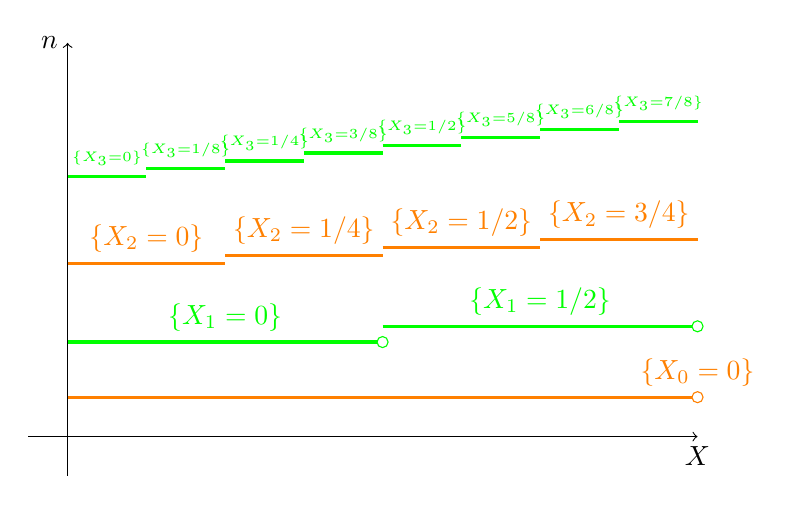
\begin{tikzpicture}
        \draw[->] (-0.5, 0)--(8, 0) node [below] {$X$};
        \draw[->] (0, -0.5)--(0, 5) node [left] {$n$};

        \draw[orange, very thick] (0, 0.5)--(8, 0.5) node [above] {$\{X_0=0\}$};
        \filldraw[color=orange, fill=white] (8, 0.5) circle (2pt);

        \draw[green, very thick] (0, 1.2)--(4, 1.2) node [midway, above] {$\{X_1=0\}$};
        \draw[green, very thick] (4, 1.4)--(8, 1.4) node [midway, above] {$\{X_1=1/2\}$};
        \filldraw[color=green, fill=white] (4, 1.2) circle (2pt);
        \filldraw[color=green, fill=white] (8, 1.4) circle (2pt);

        \draw[orange, very thick] (0, 2.2)--(2, 2.2) node [midway, above] {$\{X_2=0\}$};
        \draw[orange, very thick] (2, 2.3)--(4, 2.3) node [midway, above] {$\{X_2=1/4\}$};
        \draw[orange, very thick] (4, 2.4)--(6, 2.4) node [midway, above] {$\{X_2=1/2\}$};
        \draw[orange, very thick] (6, 2.5)--(8, 2.5) node [midway, above] {$\{X_2=3/4\}$};

        \draw[green, very thick] (0, 3.3)--(1, 3.3) node [midway, above] {$\scriptscriptstyle\{X_3=0\}$};
        \draw[green, very thick] (1, 3.4)--(2, 3.4) node [midway, above] {$\scriptscriptstyle\{X_3=1/8\}$};
        \draw[green, very thick] (2, 3.5)--(3, 3.5) node [midway, above] {$\scriptscriptstyle\{X_3=1/4\}$};
        \draw[green, very thick] (3, 3.6)--(4, 3.6) node [midway, above] {$\scriptscriptstyle\{X_3=3/8\}$};
        \draw[green, very thick] (4, 3.7)--(5, 3.7) node [midway, above] {$\scriptscriptstyle\{X_3=1/2\}$};
        \draw[green, very thick] (5, 3.8)--(6, 3.8) node [midway, above] {$\scriptscriptstyle\{X_3=5/8\}$};
        \draw[green, very thick] (6, 3.9)--(7, 3.9) node [midway, above] {$\scriptscriptstyle\{X_3=6/8\}$};
        \draw[green, very thick] (7, 4)--(8, 4) node [midway, above] {$\scriptscriptstyle\{X_3=7/8\}$};
      \end{tikzpicture}\end{center}
      Moim zdaniem to już pokazuje równość. Dowolny zbiór z $RHS$ wystarczy rozbić na wystarczająco dużo (nadal przeliczalnie) zbiorów postaci $[k 2^{-n}, (k+1)2^{-n})$ dla odpowiednich $n$. Przejście z $RHS$ do $LSH$ jest nawet bardziej trywialne, bo każdy zbiór z $\sigma(X_n)$ można zapisać jako $\{X\in B\}$ dla $B\in Bor[0, 1)$ tak jak na obrazku wyżej.
    \item Tak jak już ustaliliśmy w poprzednim podpunkcie, wiemy, że zbiory z ciała $\set{F}_n$ są generowane przez zdarzenia $\{X\in[k2^{-m}, (k+1)2^{-m})\}$ dla $m=0,1,..., n$ i $k=0,1,...,2^m-1$. Weźmy więc jeden z takich zbiorów $A=\{X\in[k2^{-m}, (k+1)2^{-m}\}\in\set{F}_n$ i popatrzmy jak powinno wyglądać wwo
      \begin{align*}
        \expected{\expected{h(X_{n+1})}{\set{F}_n}\mathds{1}_A}&=\expected{h(X_{n+1})\mathds{1}_A}
      \end{align*}
      Zauważmy, że jeśli $n+1=m+l$, to $X_{n+1}$ ma $2^l$ segmentów na $A$, tzn.
      $$X_{n+1}\mathds{1}_{\{X\in[k2^{-m}, (k+1)2^{-m})\}}=\sum_{i=0}^{2^l-1}X_n\mathds{1}_{\{X\in [k2^{-m}+i2^{-(n+1)}, k2^{-m}+(i+1)2^{-(n+1)}\}}$$
      i na każdym ze zbiorów $\{X\in[k2^{-m}+i2^{-(n+1)}. k2^{-m}+(i+1)2^{-(n+1)})\}$ zmienna $X_n$ przyjmuje wartość $k2^{-m}+i2^{-(n+1)}$. Mając tę wiadomość z tyłu głowy, możemy wrócić do szukania wwo.
      \begin{align*}
        \expected{h(X_{n+1})\mathds{1}_A}&=\expected{\sum_{i=0}^{2^l-1}h(X_{n+1})\mathds{1}_{\{X\in[k2^{-m}+2^{-(n+1)}, k2^{-m}+(i+1)2^{-(n+1)})\}}}=\\ 
                                         &=\expected{\sum_{i=0}^{2^l-1}h(k2^{-m}+i2^{-(n+1)})\mathds{1}_{\{X\in[k2^{-m}+i2^{-(n+1)}, k2^{-m}+(i+1)2^{-(n+1)})\}}}=\\ 
                                         &=\sum_{i=0}^{2^l-1}h(k2^{-m}+i2^{-(n+1)})\prob{X\in[k2^{-m}+i2^{-(n+1)}, k2^{-m}+(i+1)2^{-(n+1)})}=\\
                                         &=\sum_{i=0}^{2^l-1}h(k2^{-m}+i2^{-(n+1)})2^{-(n+1)}
      \end{align*}
      z drugiej strony, policzmy $\expected{1/2(h(X_n) + h(X_n+2^{-(n+1)})\mathds{1}_A}$
      \begin{align*}
        \expected{1/2(h(X_n) + h(X_n+2^{-(n+1)})\mathds{1}_A}=&\frac{1}{2}[\expected{h(X_n)\mathds{1}_A}+\expected{h(X_n+2^{-(n+1)})} ]=\\ 
                                                             =&\frac{1}{2}\sum_{i=0}^{2^{l-1}-1}2^{-n}h(k2^{-m}+i2^{-n})+\\ 
                                                              &+\frac{1}{2}\sum_{i=0}^{2^{l-1}-1}2^{-n}h(k2^{-m}+i2^{-n}+2^{-(n+1)})=\\ 
                                                             =&\sum_{i=0}^{2^{l-1}-1}2^{-(n+1)}h(k2^{-m}+(2i)2^{-(n+1)})+\\ 
                                                              &+\sum_{i=0}^{2^{l-1}-1}2^{-(n+1)}h(k2^{-m}+(2i+1)2^{-(n+1)})
      \end{align*}
      pierwszy wyraz odpowiada za parzyste fragmenty $\expected{h(X_{n+1})\mathds{1}_A}$, a drugi odpowiada za nieparzyste. Stąd mogę powiedzieć, że
      $$\expected{h(X_{n+1})}{\set{F}_n}=1/2[h(X_n)+h(X_n+2^{-(n+1)})]$$
      Jeśli teraz stwierdzimy, zamiast $h$ podstawimy $f(X_n+2^{-n})-f(X_n)$, co jest ograniczone przez $L2^{-n}\leq L$ z definicji funkcji $f$ (ale nie jestem świadoma gdzie konkretnie używałam ograniczoności $h$, może żeby wyciągnąć sumę przed całkę?), dostajemy
      %(bo chyba nie korzystałam z ograniczoności $h$), to dostajemy
      \begin{align*}
        \expected{Z_{n+1}}{\set{F}_n}&=\expected{2^{n+1}[f(X_{n+1}+2^{-(n+1)})-f(X_{n+1})]}{\set{F}_n}=\\ 
                                     &=2^{n+1}[\expected{f(X_{n+1}+2^{-(n+1)})}{\set{F}_n}-\expected{f(X_{n+1})}{\set{F}_n}]=\\ 
                                     &=2^{n+1}[1/2[{\color{blue}f(X_n+2^{-(n+1)})}+f(X_n+2\cdot2^{-(n+1)})]-1/2[f(X_{n})+{\color{blue}f(X_n+2^{-(n+1)})}]]=\\ 
                                     &=2^n[f(X_n+2^{-n})-f(X_n)]=Z_n
      \end{align*}
    \item Nie mam pojęcia jak to zrobić, ale z twierdzenia Dooba o zbieżności martyngałów wiemy, że istnieje zmienna losowa całkowalna $Z$ taka, że $Z_n\to Z$, bo
      $$\sup \expected{Z_n^+}=\sup\expected{2^n(f(X_n+2^{-n})-f(X_n))}\leq \sup \expected{2^nL|(X_n+2^{-n})-X_n|}=\sup\expected{L}=L<\infty.$$
      Ale przecież $Z_n=g(X_n)$ dla pewnej funkcji ograniczonej $g$ (jak wyżej), czyli $\lim Z_n=\lim g(X_n)=g(X)$, bo $X_n\to X$.
  \end{enumerate}
\end{solution}

\begin{problem}
  Niech $X_n$ będzie ciągiem zmiennych losowych przyjmujących wartości w $[0,1]$ takim, że $X_0=a\in[0,1]$. Dla $n\in\N$ niech $\set{F}_n=\sigma(X_1,X_2,...,X_n)$. Załóżmy, że
  $$\prob{X_{n+1}=X_n/2}{\set{F}_n}=1-X_n,\quad \prob{X_{n+1}=(1+X_n)/2}{\set{F}_n}=X_n$$
  \begin{enumerate}[label=(\alph*)]
    \item Pokaż, że $(X_n)$ jest martyngałem. Wywnioskuj, że $X_n$ jest zbieżne p.w. do pewnej zmiennej losowej $Z$.
    \item Pokaż, że $4\expected{(X_{n+1}-X_n)^2}=\expected{X_n(1-X_n)}$
    \item Znajdź rozkład zmiennej losowej $Z$
  \end{enumerate}
\end{problem}

\begin{solution}
\end{solution}

